\documentclass[25pt, a0paper, portrait]{tikzposter}

\usepackage[compress]{cite}

\usepackage{parskip}
\usepackage{amssymb}
\usepackage{stix}
\usepackage{amsmath}
\usepackage{mathtools}
\usepackage{multirow}
\usepackage{graphicx}
\usepackage{xstring}
\usepackage{etoolbox}
\usepackage{notoccite}
\usepackage{natbib}
\usepackage{mathrsfs}
\usepackage{lineno}
\usepackage{tensor}
\usepackage{accents}
\usepackage{capt-of}
\usepackage{tabularx}
\usepackage{tikz}
\usetikzlibrary{shapes.arrows}
\allowdisplaybreaks
% Use Envelope theme
\usetheme{Envelope}

\tikzposterlatexaffectionproofoff{}

\let\oldbibliography\thebibliography
\renewcommand{\thebibliography}[1]{\oldbibliography{#1}
\setlength{\itemsep}{-3pt}} %Reducing spacing in the bibliography.

\pdfinclusioncopyfonts=1 % Fix fonts on non-linux machines


% Custom colors
\definecolor{myPink}{RGB}{255,182,193}
\definecolor{myDarkPink}{RGB}{220,38,127}
\definecolor{myPurple}{RGB}{120,94,240}
\definecolor{myOrange}{RGB}{254, 97, 0}
\definecolor{myYellow}{RGB}{245, 176, 0}
\definecolor{myBlue}{RGB}{100, 143, 255}

% Set colors
\colorlet{backgroundcolor}{myPink}
\colorlet{framecolor}{myPurple}
\colorlet{titlebgcolor}{myPurple}
\colorlet{titlefgcolor}{white}
\colorlet{blocktitlebgcolor}{myDarkPink}
\colorlet{innerblocktitlebgcolor}{myPurple}


% Title, author, etc.
\title{\parbox{\linewidth}{\centering Poincaré Gauge Theory versus Cosmological Tensions}}
\author{Sinah Legner <sl2091@cam.ac.uk>, Will Handley <wh260@cam.ac.uk>, Will Barker <wb263@cam.ac.uk>}
\institute{University of Cambridge $\cdot$ Kavli Institute for Cosmology $\cdot$ Cavendish Laboratory}

\makeatletter
\renewcommand\TP@maketitle{%
    \centering
    \vspace{-40pt}
    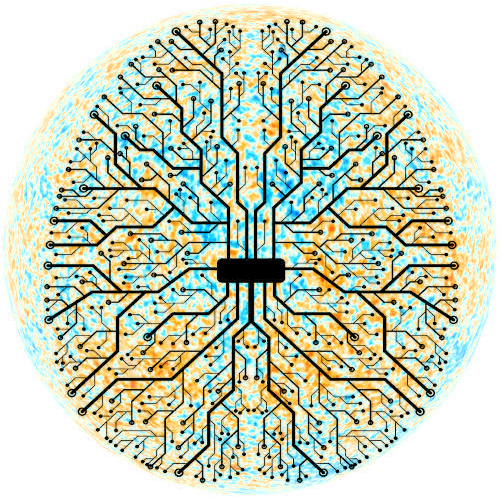
\includegraphics[height=0.11\textwidth]{handley-lab.png}\hfill
    \begin{minipage}[b]{0.7\linewidth}
        \centering
        \color{titlefgcolor}
        \vspace*{1em}
        {\bfseries \Huge \fontsize{100}{120} \sc \@title \par}
        \vspace*{1em}
        % {\huge \@author \par}
        \vspace*{1em}
         % {\LARGE \@institute}
    \end{minipage}%
    \hfill
\includegraphics[height=0.11\textwidth]{cambridge-cropped.pdf}
}
\makeatother

% Begin document
\begin{document}
\maketitle
% Block style
\tikzstyle{Block} = [rectangle, draw, fill=myPink, rounded corners, shade, inner sep=10pt]

% Envelope-themed block
\block{}{
\begin{minipage}{0.1\textwidth}
    \begin{tikzfigure}
    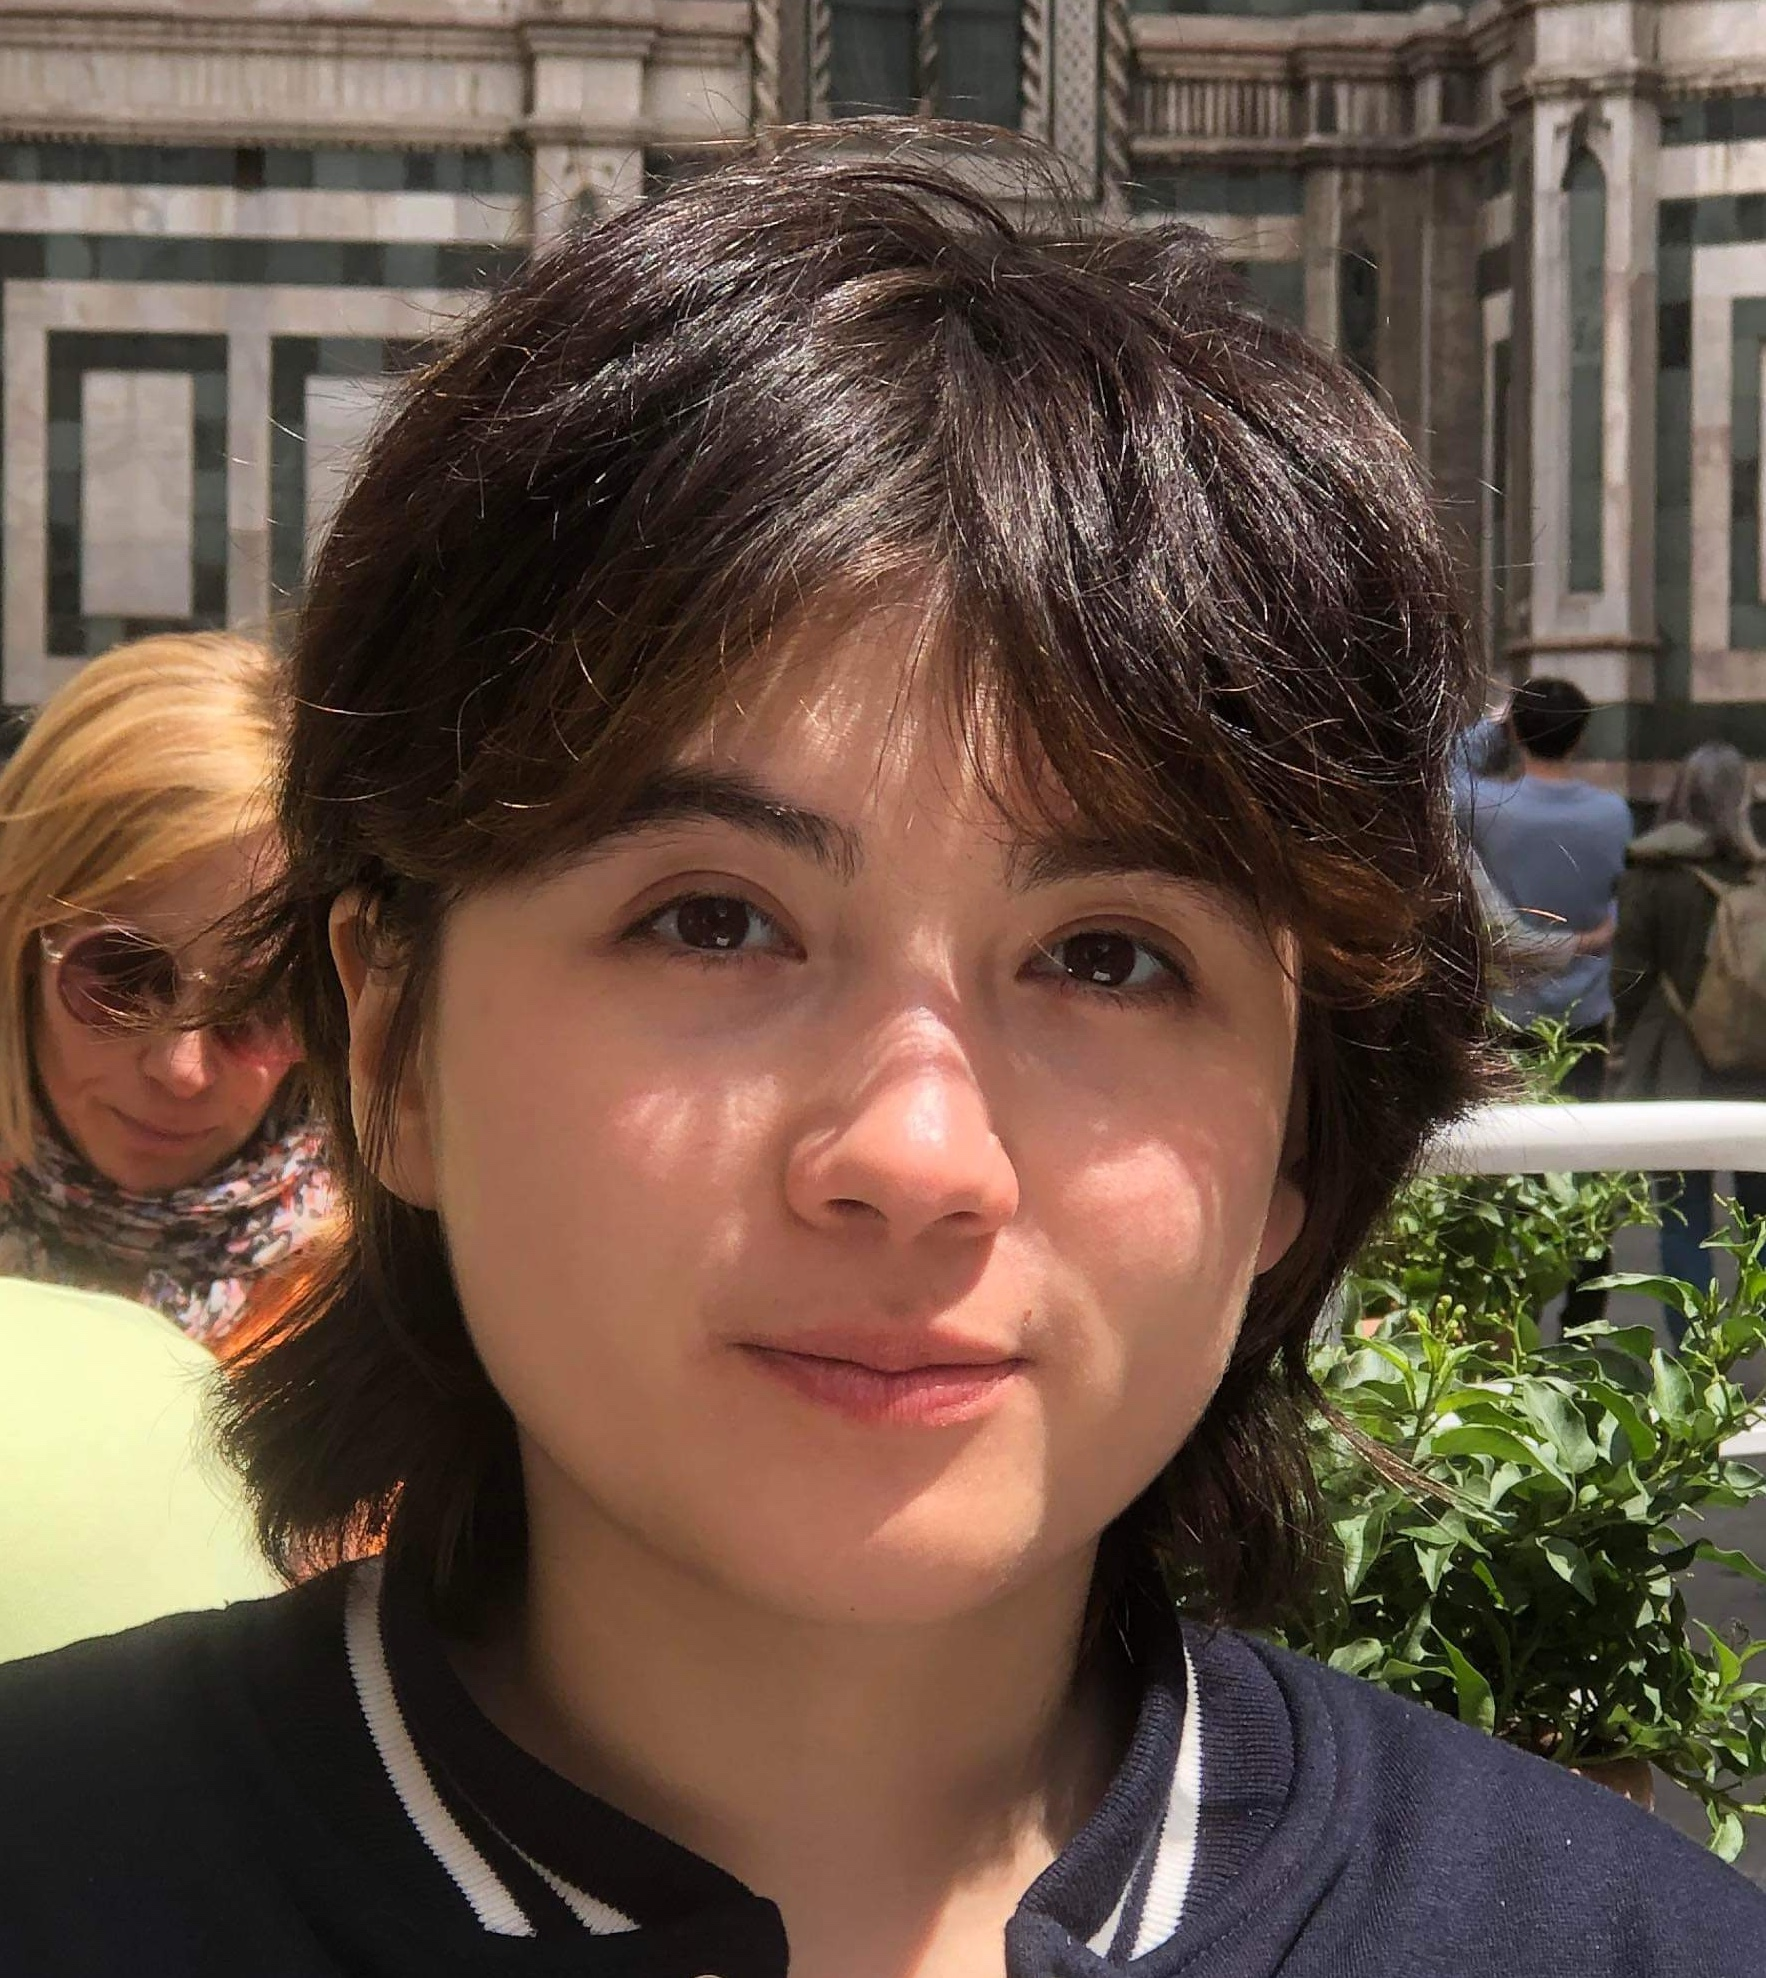
\includegraphics[width = 0.9\textwidth]{me.JPG}
    \end{tikzfigure}
\end{minipage}
\begin{minipage}{0.19\textwidth}
\innerblock{}{\begin{tabularx}{\linewidth}{@{}lX@{}}
    Author: &\textbf{Sinah Legner} \\
            & <sl2091@cam.ac.uk> \\
    Co-Authors: &\textbf{Will Handley}  \\
            &<wh260@cam.ac.uk> \\
            & \textbf{Will Barker} \\
            &<wb263@cam.ac.uk> 
    \end{tabularx}
    }
\end{minipage}
\hspace{0.2cm}
\begin{minipage}{0.53\textwidth}
We present the Poincaré Gauge Theory (PGT) of gravity~\cite{Barker:2020gcp, Barker:2020elg}, focusing on constant torsion emergent gravity (CTEG), a specific case of PGT which coincides with $\Lambda$CDM under specific parameter choices.
The difference between CTEG and GR is absorbed through a redefinition of the dark energy equation of state. Using CAMB~\cite{2011ascl.soft02026L}, Polychord~\cite{Handley_2015}, and Cobaya~\cite{Torrado_2021}, the constraints on the cosmological parameters under CTEG cosmology are derived. Our analysis compares CTEG with $\Lambda$CDM, showing that although fixing the parameters in CTEG results in a higher value of $H_0$, this is not favoured by data.
\end{minipage}
\begin{minipage}{0.1\textwidth}
    \begin{tikzfigure}
    
\includegraphics[width = \textwidth]{kicc.png}
\end{tikzfigure}
\end{minipage}
}

\begin{columns}
    \column{0.5}
    \block{1. Poincare Gauge Theory (PGT)}{        
        \vspace{3cm}
        \hspace{7cm}
        \begin{minipage}{0.43\textwidth}
        \begin{tikzpicture}
        \node{
            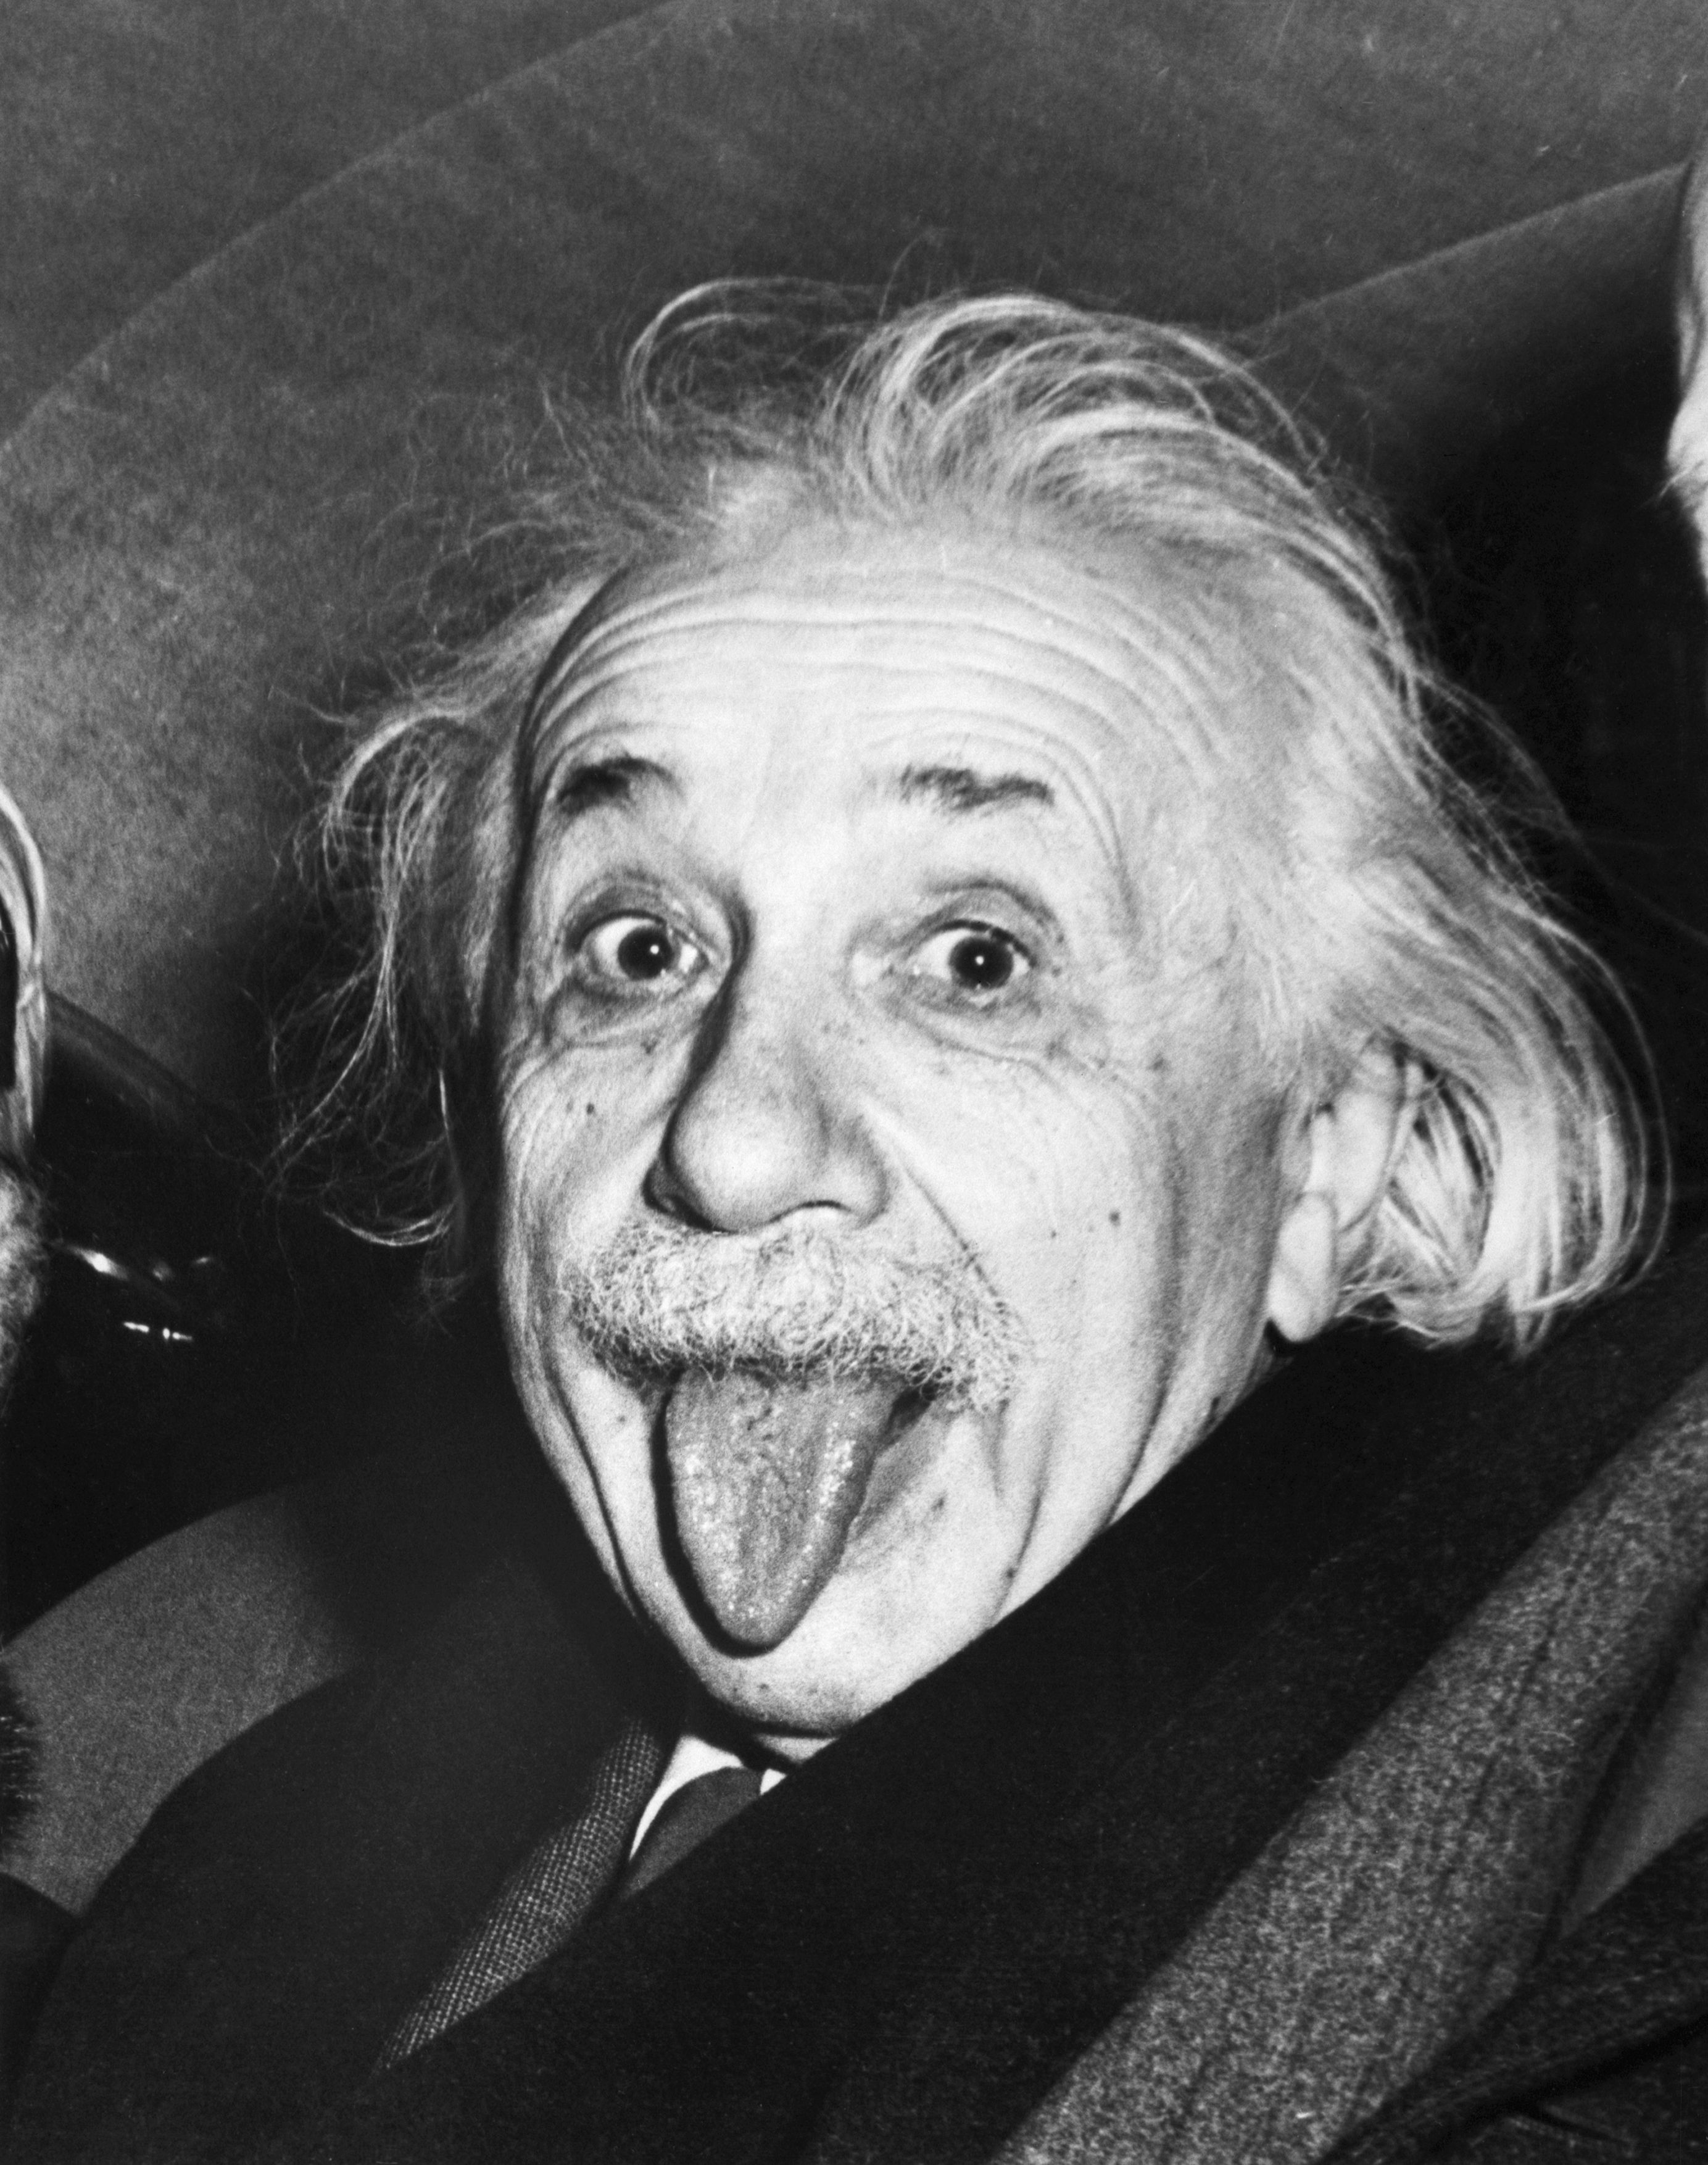
\includegraphics[width=0.3\textwidth]{albert-einstein-sticks-out-his-tongue-when-asked-by-news-photo-1681316749.jpg}
            \node[ellipse callout, inner sep= 0pt, fill=myYellow, aspect=2.5,  text width=8cm, text centered, xshift=-11cm, yshift=15cm, callout relative pointer={(0.8,-2)}] at (0,0)        {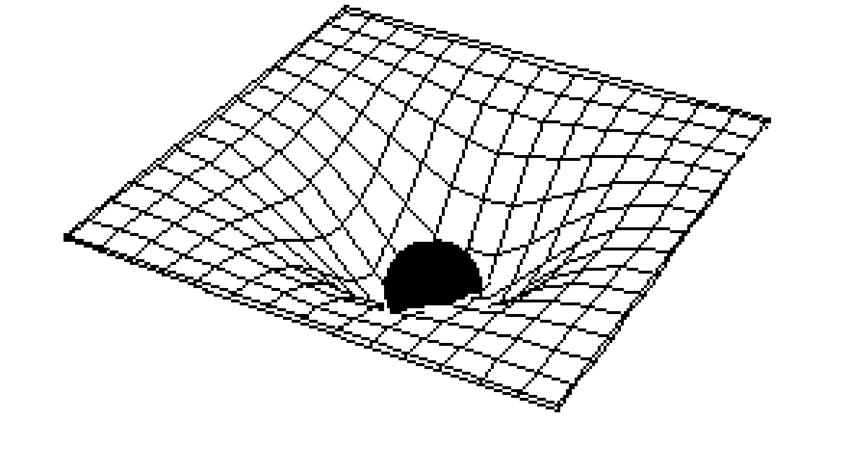
\includegraphics[width=\textwidth]{Space-in-the-presence-of-an-object-with-mass.png}};
            \node[text width=8cm, text centered, xshift=-7cm, yshift=16cm]{\small~\cite{article}}
            \draw[myDarkPink, line width=5mm] (-13,17) -- (0,-0.5);
            \draw[myDarkPink, line width=5mm] (-13,-0.5) -- (0,17);
            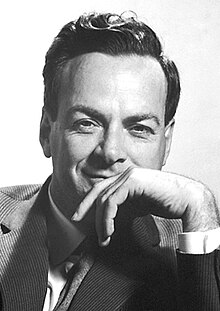
\includegraphics[width=0.28\textwidth]{Richard_Feynman_Nobel.jpg}
            \node[cloud callout, inner sep= 0pt, fill=myYellow, aspect=2.5,  cloud puff arc=120, text width=8cm, text centered, xshift=0cm, yshift=15cm, callout relative pointer={(-0.5, -2)}] at (0,0) {\huge Gauge Theory};
        \end{tikzpicture}
        }
        \vspace{0.5cm}
        \end{minipage}
            \begin{itemize}
            \item  Poincaré Gauge Theory (PGT):  how Feynman would construct gravity, not as curvature of spacetime, but as a gauge field theory similar to other forces in quantum field theory.
            \item  Constant Torsion Emergent Gravity (CTEG): a specific ghost-free, tachyon-free, and renormalisable PGT with second-order equations of motion, screened from curvature.
        \end{itemize}
        \vspace{0.5cm}
    \innerblock{CTEG Lagrangian density}{%
            \begin{align*}
                \mathcal{L} &= \text{M}_\text{p}^2 \left[ \frac{2}{3}\left(\frac{\varpi^2}{4 }-1\right) \mathcal{R} + \partial_\mu \varpi \partial^\mu \varpi
                -\frac{4}{3}\sqrt{|J_{\mu } J^{\mu }|}-
               \phi ^2+ \phi ^2 \varpi ^2 \right] ,\\
                J_{\mu} & =  4 \varpi^3 \partial_{\mu} (\phi/\varpi) + \partial_{\mu} \phi , \;\;\;\;\;\; \phi  =  \frac{2 H (\varpi^2 - 1)+\varpi \, \dot{\varpi}}{\varpi^2-1} .
            \end{align*}
        }
    }
    
    % \note[targetoffsetx=11cm,targetoffsety=-15cm, connection,angle=-20,radius=0.08\textwidth]{Expression of $\phi$ is obtained through its equation of motion}
    
    \block{3. Method}{
        \begin{minipage}{0.22\textwidth}
            \innerblock{$\Omega_{\Lambda, \mathrm{eff}}(t)$ in CAMB}{
            
            \[ \scalebox{2}{$\displaystyle \Omega_\Lambda e^{-3 \int (1+\mathcolor{myDarkPink}{w_{\mathrm{eff}}(a)}) d \ln a}$} \]
            }
            
        \end{minipage}
        \begin{minipage}{0.22\textwidth}
            \begin{itemize}
                \item Effects of extra parameters on Cosmology are absorbed into redefinition of $w_{\mathrm{eff}}(a)$ and input into CAMB.
                \item $\Omega_\Lambda$ in CAMB is a constant derived from $\Omega_\Lambda = 1-\sum^{i \neq \Lambda}\Omega_i$.
            \end{itemize}
        \end{minipage}
        
        \vspace{0.5cm}
        \begin{minipage}{0.19\textwidth}
            \begin{itemize}
                \item Cosmological run is performed through Cobaya, with PolyChord sampler and Planck 2018 likelihood.
                \item Poles in $w_{\mathrm{eff}}$ give constraints on the priors of the CTEG parameters.
            \end{itemize}
        \end{minipage}
        \begin{minipage}{0.12\textwidth}
            \innerblock{Priors}{
            \begin{align*}
                0.6 < &\, \varpi_r < 1 \\
                0 < &\, \Omega_L < 1-\Omega_m
            \end{align*}
            }
        \end{minipage}
        \begin{minipage}{0.13\textwidth}
            \innerblock{GR-Coincident Values}{
            \begin{align*}
                \varpi_r & = 1 \\
                \Omega_L & = \Omega_\Lambda
            \end{align*}
            }
        \end{minipage}
    }
    

    \block{5.Conclusion}{
        \begin{tikzfigure}
            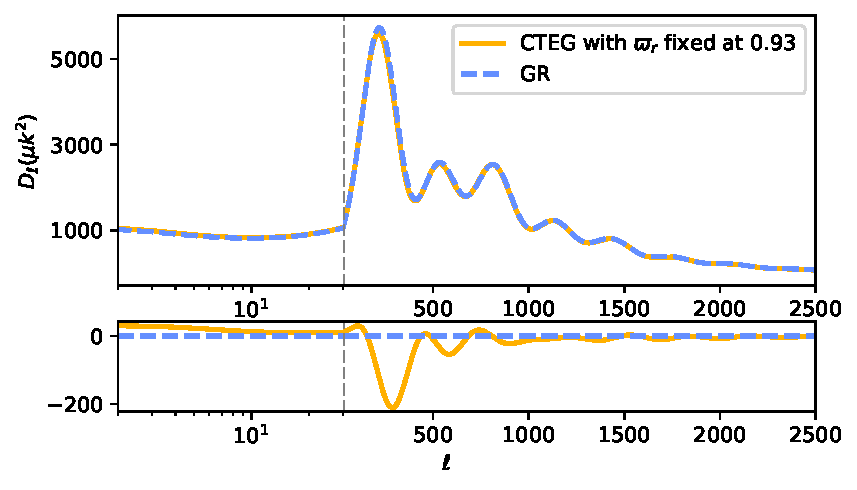
\includegraphics[width=0.42\textwidth]{resplot.pdf}
        \end{tikzfigure}
    \begin{itemize}
         \item Artifically fixing $\varpi_r$ to a lower value, such as 0.93, results in a higher value of $H_0$.
         \item However, this result is not preferred by data: when $\varpi_r$ is a free parameter, it tends towards the GR-coincident value $\varpi_r \rightarrow 1$, indicating that the data favours $\Lambda$CDM.
         \item CMB power spectrum plotted from the best fit parameters of CTEG with $\varpi_r = 0.93$ indeed shows a discrepancy from Planck 2018 data.
         \item Cosmological theories proposed to resolve tensions should be tested with data.
     \end{itemize}
    }

    
    \column{0.5}
    \block{2. CTEG and its Parameters }{
        \innerblock{Time-dependent Dark Energy Field Equations}{
        \begin{align*}
            H^2  = & H_0^2 \left(\Omega_{r} a^{-4} +\Omega_m a^{-3} + \Omega_{\Lambda, \mathrm{eff}}(t)\right), \\
            H^2 + \partial_t H^2 = &- H_0^2\Big(\Omega_r a^{-4} +\frac{1}{2}\Omega_m a^{-3} + \Omega_{\Lambda, \mathrm{eff}}(t) \, \bigl(1+3 w_{\mathrm{eff}}(t)\bigr) \Bigr) .
        \end{align*}
        }
        \vspace{1cm}
        \innerblock{CTEG Field Equations}{
        \begin{align*}
            H^2  = & \frac{H_0^2}{\varpi^2} \Bigl(\Omega_r a^{-4}+\Omega_m a^{-3}+\Omega_L \Bigr) - \frac{\partial_t \varpi}{3 \varpi^2} \biggl(6 H \varpi + \frac{\left(1+3\varpi^2\right)\partial_t \varpi}{\varpi^2-1}\biggr), \\
            \partial_t^2 \varpi = & \frac{1}{\left(\varpi^2-1\right)\left(3 \varpi^2 +1\right)}\Bigl( -3 \varpi \left(\varpi^2 -1\right)^2 \left(2 H^2 + \partial_t H\right) \\
            & + 3 H \left(1 + 2 \varpi^2 - 3 \varpi^4\right) \partial_t \varpi + 4 \varpi \partial_t \varpi^2 \Bigr).
        \end{align*}
        }
        \begin{tikzpicture}[overlay]
            \node[single arrow, draw=myDarkPink, fill=myDarkPink, 
          minimum width = 4cm, single arrow head extend=0.3cm,
          minimum height=3cm,
          rotate=270, xshift=-13.2cm, yshift=5cm] {};   
        \end{tikzpicture}
        
        \begin{minipage}{0.27\textwidth}
            \begin{itemize}
                \item CTEG cosmology is solved by propagating field equations from early time, using power series.
                \item Evolution of both scale factor $a$ and scalar field $\varpi$ are determined by initial value of $\varpi$, defined as $\varpi_r$.
                \item Bare dark energy density $\Omega_L$ is modified such that $H = H_0$ at today's time $t_0$. 
            \end{itemize}
        \end{minipage}\hspace{1cm}
        \begin{minipage}{0.16\textwidth}
            \coloredbox[bgcolor = myYellow, framecolor = myYellow]{
            \begin{tabularx}{\linewidth}{@{}lX@{}}
                $\mathbf{\varpi_r}$ : & Initial condition of $\varpi$ at early time\\
                
                $\mathbf{\Omega_L}$ : & Energy density parameter of bare dark energy
            \end{tabularx}
            }
        \end{minipage}

    }
%     \vspace{2cm}
%     \begin{align*}
%         H^2  & = && H_0^2 \Bigl(\Omega_{r} a^{-4} +\Omega_m a^{-3} + \Omega_{\Lambda}^{\mathrm{eff}}(t)\Bigr) && = && \frac{H_0^2}{\varpi^2} \Bigl(\Omega_r a^{-4}+\Omega_m a^{-3}+\Omega_L \Bigr) \\
%         & && && &&- \frac{\partial_t \varpi}{3 \varpi^2} \biggl(6 H \varpi + \frac{\left(1+3\varpi^2\right)\partial_t \varpi}{\varpi^2-1}\biggr)\\
%         H^2 + \partial_t H^2 & = && - H_0^2\Big(\Omega_r a^{-4} +\frac{1}{2}\Omega_m a^{-3}  && = && - \frac{H_0^2}{\varpi^2}\Bigl(\Omega_r a^{-4} + \frac{1}{2}\Omega_m a^{-3} - \Omega_L\Bigr)\\
%         & && + \Omega_{\Lambda}^{\mathrm{eff}}(t) \, \bigl(1+3 w_{\Lambda}^{\mathrm{eff}}(t)\bigr) \Bigr) && && - \frac{1}{3 \varpi^2}\biggl(3 H \varpi \partial_t \varpi - \frac{(5+3 \varpi^2) \partial_t \varpi ^2}{\varpi -1}\\
%         & && && &&+ 3 \varpi \partial_t^2 \varpi\biggr)
%     \end{align*}
%     \begin{tikzpicture}[overlay]
%     % Define the coordinates for the frame
%     \draw[myPurple, line width=1.5mm] (6.5, 0) rectangle (20, 15);
    
%     % Optional: Add content within the frame
%     \node at (6.5, 15) {Time-dependent Dark Energy Field Equations};
% \end{tikzpicture}
    
    
    \block{4. Cosmological Run Result}
    {
        \begin{tikzfigure}
            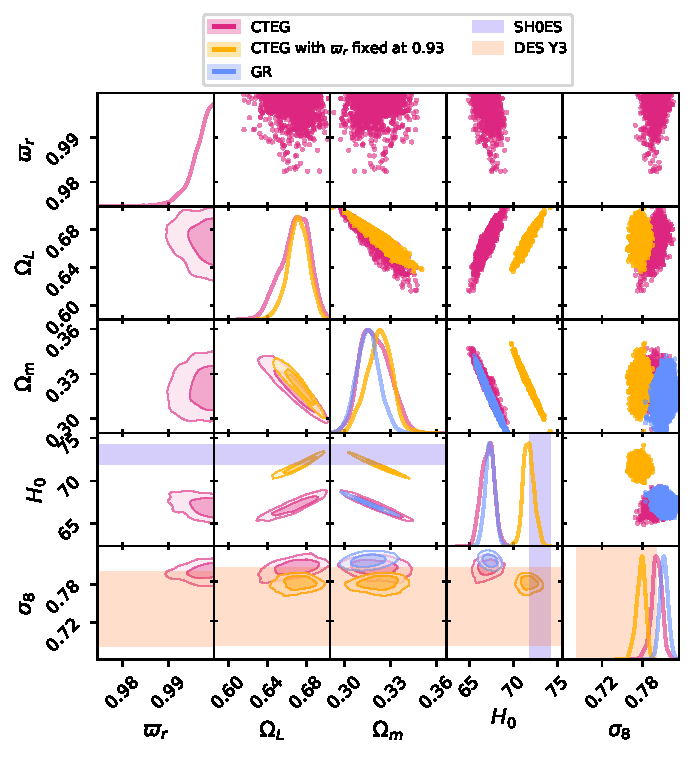
\includegraphics[width=0.38\textwidth]{corner.pdf}
            Cosmological results of CTEG and CTEG with $\varpi_r$ fixed at 0.93, compared with $\Lambda$CDM result from Planck 2018~\cite{planck2018}. Figure also showing $H_0$ from SH0ES~\cite{Riess_2022}, and $\sigma_8$ from DES Y3~\cite{2022PhRvD.105b3520A}.
        \end{tikzfigure}
    }
    
\renewcommand{\section}[2]{}%
    \block{6. References}{
    \begin{minipage}[b]{0.36\textwidth}
    \bibliographystyle{unsrt}
    \tiny
    \bibliography{Inspirehep, Notinspire}
    \end{minipage}
    
    }

\end{columns}
\end{document}